\documentclass[a4paper]{article}
\usepackage[UTF8]{ctex}
\usepackage{geometry}
\usepackage{graphicx}
\usepackage{url}
\usepackage{multirow}
\usepackage{array}
\usepackage{booktabs}
\usepackage{url}
\usepackage{enumitem}
\usepackage{graphicx}
\usepackage{float}
\usepackage{amssymb}
\usepackage{amsmath}
\usepackage{subfig}
\usepackage{longtable}
\usepackage{pifont}
\usepackage{color}

\allowdisplaybreaks

\geometry{a4paper, scale=0.78}

\usepackage{tikz}
\newcommand*{\circled}[1]{\lower.7ex\hbox{\tikz\draw (0pt, 0pt)%
    circle (.5em) node {\makebox[1em][c]{\small #1}};}}
    

% \begin{figure}[H]
%     \centering
%     \includegraphics[width=.55\textwidth]{E.png}
%     \caption{矩阵与列向量的乘法}
%     \label{fig:my_label_1}
% \end{figure}

% \left\{
% \begin{array}{ll}
%       x+2x+z=2 & \\
%       3x+8y+z=12 & \\
%       4y+z=2
% \end{array}
% \right.

% \begin{enumerate}[itemindent = 1em, itemsep = 0.4pt, parsep=0.5pt, topsep = 0.5pt]

% \end{enumerate}

%\stackrel{a}{\longrightarrow}

%\underbrace{}_{} %下括号

%\tableofcontents %目录,并且目录页不记录页码
% \tableofcontents
% \newpage
% \setcounter{page}{1} %new page
% \clearpage

\title{Sigmoid Belief Network}
\author{Chen Gong}
\date{17 March 2020}

\begin{document}
\maketitle
%\pagestyle{empty}
\tableofcontents
\newpage
%\pagestyle{fancy}
\setcounter{page}{1} %new page
\clearpage

\section{Background}
\subsection{什么是Sigmoid Belief Network}
这一节将要学习的是Sigmoid Belief Network。首先来想一想这个名字是怎么来的,其中Belief就等价于Bayesian Network(俗称有向图),而Sigmoid指的是Sigmoid Function:
$$
\sigma(x) = \frac{1}{1+\exp{-x}}
$$
表示图中的节点都是服从0/1分布的离散随机变量,并且概率值和Sigmoid函数有关。

总所周知,有向图的因子分解很简单,因为变量之间的关系非常的清晰。而且采样也非常的简单,先从根节点开始采样,在根节点已知的情况下,子节点之间都是条件独立的(D-Separation中的Tail to Tail原则)。这样我们就可以一层一层的往下采样,而在神经网络中用足够多的隐藏层可以近似任何分布,在这里也一样,只要深度足够可以逼近任何的二值分布。

Neal在1990年结合Boltzmann Model提出了Sigmoid Belief Network。Boltzmann Machine定义了观察变量$V$和未观察变量$V$的联合分布概率:
\begin{equation}
    P(v,h) = \frac{\exp{\{-\mathrm{E}(v,h)}\}}{\sum_{v,h}\exp{\{-\mathrm{E}(v,h)}\}}
\end{equation}
而能量函数为:
\begin{equation}
    \mathrm{E}(v,h) = -\sum_i\alpha_iv_i - \sum_j\beta_jh_j - \sum_{i,j} v_i w_{ij} h_j
\end{equation}
通过调整权值可改变概率。有了联合分布概率,从而很容易得到观察变量的概率:
\begin{equation}
    P(v,h) = \frac{\sum_h\exp{\{-\mathrm{E}(v,h)}\}}{\sum_{v,h}\exp{\exp{\{-\mathrm{E}(v,h)}\}}}
\end{equation}
因为我们观测到的数据只有可观测变量,所以学习调整权值的目的就是极大化观察变量的似然函数$-\log p(V)$。

\textbf{Sigmoid Belief Network将无向图变成有向图的结构则有更好的因果(causal)形式,其中未观察变量被看作观察变量发生的原因。}

\subsection{Sigmoid Belief Network的模型表示}
假设无向图中的节点为,$\{ S_1,S_2,\cdots,S_T \}$。根据可观测变量和不可观测变量,可以划分为$\{V,H\}$。如下图所示:
\begin{figure}[H]
    \centering
    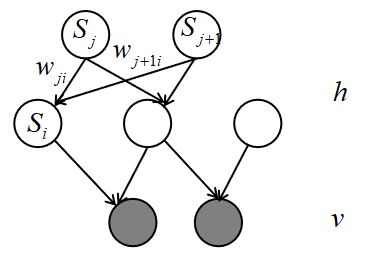
\includegraphics[width=.35\textwidth]{微信图片_20200317124813.png}
    \caption{Sigmoid Belief Network的模型概率图}
    \label{fig:my_label_1}
\end{figure}
\textbf{注意我们用$j<i$来表示i的父亲节点,在离散数学里这是一种偏序关系,我们可以简单的认为$S_j$节点在$S_i$节点之前进行采样。(这里老师讲的有点模糊,开始听的有点懵逼)}那么$S_i$节点的概率分布,等于它的两个父亲节点的分布和相应的权重的乘积之和对应的一个Sigmoid函数(Sigmoid函数就是用在这儿的),即为:
$$
P(S_i=1) = \sigma(w_{ji}S_j + w_{j+1i}S_{j+1}) = \sigma(\sum_{j<i}w_{ji}S_j )
$$
考虑到条件独立性,完整的可以写为:
\begin{equation}
    P(S_i=1|S_{j:j<i}) = \sigma\left(w_{ji}S_j + w_{j+1i}S_{j+1}\right) = \sigma\left(\sum_{j<i}w_{ji}S_j \right)
\end{equation}
那么很简单就可以表示$P(S_i=0|S_{j:j<i})$,
\begin{equation}
    P(S_i=0|S_{j:j<i}) = 1 - \sigma\left(w_{ji}S_j + w_{j+1i}S_{j+1}\right) = \sigma\left(-w_{ji}S_j + w_{j+1i}S_{j+1}\right)
\end{equation}
这里用到了一个很重要的性质,即为:$1 - \sigma(x)=\sigma(-x)$这个公式很简单,同学们自己推就可以了。下一个问题是,想把公式(4)和(5)合并一下,因为分开不好进行统一的表达。思考到当$S_i=1$时,希望系数为$1$;当$S_i=0$时,希望系数为$-1$。令:
\begin{equation}
    S^\ast_i = 2S_i -1
\end{equation}
就可以完美的实现这个结果。所以,就可以合并起来,得到$S_i$的条件概率为:
\begin{equation}
    \left\{
    \begin{array}{ll}
      P(S_i|S_{j:j<i}) = \sigma\left(S^\ast_i\sum_{j<i}w_{ji}S_j \right)& \\
      S^\ast_i = 2S_i -1 & \\
    \end{array}
    \right.
\end{equation}
\subsection{小结}
本小节讲述了SBN算法的来源,如何从Boltzmann Machine中演变而来,以及比Boltzmann先进的原因。也梳理了一下Boltzmann Machine的求解策略。然后给出了SBN的模型表示方法,这里需要注意一下$<$是一种代表父子节点关系的偏序关系。
\section{Log Likelihood Gradient}
\subsection{Learning rule}
Neal在提出这个算法的时候,给出了Learning Rule,但是很不幸的是,这个Learning Rule存在非常明显的缺陷。我先大致的说一下,就是梯度的值用MCMC来采样,这样只能应对小规模的网络,层次一多起来就不work了(Mixing time)过长,而为什么要用MCMC方法呢?因为Head to Head的问题,请看图1,在v节点被观测的情况下,h中的节点都不是条件独立的,他们之间都是相关的。那么,$P(h|v)$就很难被求出来,因为$h$之间的节点相互影响,有相交解释。

“近似推断”那一节我们已经讲过了,Learning中是需要求后验的,这里再简单描述一下。Learning的思想是令先验的Log Likelihood Function最大化,通常使用梯度上升法来解决,在求解梯度的过程中,不可避免的要求后验,因为这个梯度的计算结果就是一个关于后验分布的期望,不可避免的要从后验中采样,因为后验很复杂不能直接采样,所以要使用MCMC从后验中采样来求近似期望。

下面我们将求解Log Likelihood Gradient来让大家有一个感性的认识。大佬这里有一句话如醍醐灌顶,\textbf{推导的目的是看看具体的过程,然后对结论有一个感性的认识,对结论的来龙去脉有更好的理解,主要目的是辅助我们理解结论,而不是为了推导而推导。}

\section{Log Likelihood Function Gradient}
假设联合概率分布为:
\begin{equation}
    P(S) = \prod_i P(S_i|S_{j:j<i})
\end{equation}
而,
\begin{equation}
    \left\{
    \begin{array}{ll}
      P(S_i|S_{j:j<i}) = \sigma\left(S^\ast_i\sum_{j<i}w_{ji}S_j \right)& \\
      S^\ast_i = 2S_i -1 & \\
    \end{array}
    \right.
\end{equation}
实际上,应该是$\sigma\left(S\ast\sum_{j<i}w_{ji}S_i + b_i \right)$,还有一个偏置,了解一点机器学习的同学都知道,这个偏置是可以放到权值里的,因为可以看成是0次项对应的系数。所以,可见变量的Log Likelihood Function为:
\begin{equation}
    \mathrm{Log\ Likelihood\ Function} = \frac{1}{N} \sum_v \log P(v)
\end{equation}
实际上这个$\frac{1}{N}$是一个常数,要不要都可以。那么梯度的表达公式为:
\begin{equation}
    \frac{\partial \log P(v)}{\partial w_{ji}} = \frac{1}{P(v)} \frac{\partial P(v)}{\partial w_{ji}} = \frac{1}{P(v)} \frac{\partial \sum_h P(v,h)}{\partial w_{ji}} = \frac{1}{P(v)} \frac{\sum_h \partial P(v,h)}{\partial w_{ji}}
\end{equation}
而$P(v)$和$h$变量没什么关系,所以,可以放到求和符号里面:
\begin{equation}
    \frac{1}{P(v)} \frac{\sum_h \partial P(v,h)}{\partial w_{ji}} = \sum_h \frac{\partial P(v,h)}{P(v) \partial w_{ji}}
\end{equation}
根据贝叶斯公式可得$P(v,h) = P(v)P(h|v)$。所以,log似然梯度为:
\begin{equation}
     \sum_h \frac{P(h|v)}{P(h,v)} \frac{\partial P(v,h)}{\partial w_{ji}} 
\end{equation}
而$P(v,h) = P(S)$,所以梯度表达为:
\begin{equation}
    \sum_h P(h|v)\frac{1}{P(S)} \frac{\partial P(S)}{\partial w_{ji}} 
\end{equation}
而$P(S) = \prod_k P(S_k|S_{j:j<k})$。而在,$P(S) = \prod_k P(S_k|S_{j:j<k})$中只有一项是和$w_{ji}$相关的。只有当$k=i$,才会对应$w_{ji}$,所以只有一项和$w_{ji}$相关。那么,梯度进一步推导为:
\begin{equation}
\begin{split}
    \sum_h P(h|v)\frac{1}{P(S)} \frac{\partial P(S)}{\partial w_{ji}} = &  \sum_h P(h|v) \frac{1}{\prod_k P(S_k|S_{j:j<k})}\frac{\partial P(S_i|S_{j:j<i})  \prod_{k\neq i} P(S_k|S_{j:j<k})}{\partial w_{ji}} \\
    = & \sum_h P(h|v) \frac{1}{P(S_i|S_{j:j<i})  \prod_{k\neq i} P(S_k|S_{j:j<k})}\frac{\prod_{k\neq i} P(S_k|S_{j:j<k}) \partial P(S_i|S_{j:j<i})}{\partial w_{ji}} \\
    = & \sum_h P(h|v) \frac{1}{P(S_i|S_{j:j<i})}\frac{ \partial P(S_i|S_{j:j<i})}{\partial w_{ji}}
\end{split}
\end{equation}
而$P(S_i|S_{j:j<i}) = \sigma\left(S^\ast_i\sum_{j<i}w_{ji}S_j \right) $。并且Sigmoid函数有一个很好的性质:
\begin{equation}
    \sigma'(x) = \frac{e^{-x}}{(1+e^{-x})^2} = \frac{1}{1+e^{-x}} \cdot \frac{e^{-x}}{1+e^{-x}} = \sigma(x)(1-\sigma(x)) = \sigma(x) \sigma(-x)
\end{equation}
\textbf{而为了方便区分,后面在$\sigma$函数中用$k$来表示$j$(这里老师直接在最后说的,我仔细回想时有点晕,我提前就换过来了,希望可以帮助到同学们)。}那么,$\frac{\partial \sigma\left(S^\ast_i\sum_{k<i}w_{ki}S_k\right)}{\partial w_{ji}} = S^\ast_i S_j $,所以:
\begin{equation}
    \begin{split}
        \sum_h P(h|v) \frac{1}{P(S_i|S_{k:k<i})}\frac{ \partial P(S_i|S_{k:k<i})}{\partial w_{ji}} = & \sum_h P(h|v) \frac{1}{\sigma\left(S^\ast_i\sum_{k<i}w_{ki}S_k \right)}\sigma\left(S^\ast_i\sum_{k<i}w_{ki}S_k \right)\sigma\left(-S^\ast_i\sum_{k<i}w_{ki}S_k \right)S^\ast_i S_j \\
        = & \sum_h P(h|v) \sigma\left(-S^\ast_i\sum_{k<i}w_{ki}S_k \right)S^\ast_i S_j
    \end{split}
\end{equation}


刚刚求得的结果总结一下为:
\begin{equation}
     \frac{\partial \log P(v)}{\partial w_{ji}} = \sum_h P(h|v) \sigma\left(-S^\ast_i\sum_{k<i}w_{ki}S_k \right)S^\ast_i S_j
\end{equation}

那么最终log Likelihood Function Gradient的结果为:
{\color{red}
\begin{equation}
    \begin{split}
        \frac{\partial}{\partial w_{ji}} \sum_v \log P(v) = & \sum_v \sum_h P(h|v) \sigma\left(-S^\ast_i\sum_{k<i}w_{ki}S_k \right)S^\ast_i S_j \\
    \end{split}
\end{equation}
}
而$P(h|v)$可以被写作$P(h,v|v) = P(S|v)$。所以,$\sum_v \sum_h P(h|v) = \sum_S P(S|v)$。那么,梯度可以写为:
\begin{equation}
    \begin{split}
        \frac{\partial}{\partial w_{ji}} \sum_v \log P(v) = & \sum_S P(S|v) \sigma\left(-S^\ast_i\sum_{k<i}w_{ki}S_k \right)S^\ast_i S_j \\
        = & \mathbb{E}_{(v,h)\sim P(S|v),\ v\sim P_{\mathrm{data}}}\left[ \sigma\left(-S^\ast_i\sum_{k<i}w_{ki}S_k \right)S^\ast_i S_j \right]
    \end{split}
\end{equation}
其中,$S_i$代表的是第$i$个节点的随机变量,这就是Neal提出的Sigmoid Belief Network的Learning Rule。在学习的梯度迭代的过程中,是很依赖后验分布的。所以,如何把$\sum_s P(S|v)$求出来是个大问题,后验概率分布非常的重要,但是这是求不出来的。在观测变量已知的情况下,由于D-Separation中的Head to Head问题,导致所有节点之间都是有联系的,没有条件独立性,关系太复杂了。所以,$\sum_s P(S|v)$过于复杂,无法之间求解。Neal提出的这种方法用MCMC来近似计算$P(S|v)$很显然只适合于小规模的图,一旦复杂起来就会出现Mixing time过长的问题,根本就不work。

\subsection{小结}
我们在这一小节中,讲述了Neal提出来的learning rule,说白了就是如何使Log Likelihood Function最大化,那么就要求它的梯度。梯度的表达式,为一个关于后验的期望,由D-Separation原则可知,后验分布过于复杂,无法求解。
用MCMC来近似计算,然而这样的方法只适合于小规模的图,一旦复杂起来就会出现Mixing time过长的问题。所以,需要寻找新的方法。

\section{Wake-Sleep Algorithm}
小编在理解这个算法的过程中是有点艰辛的,主要是小编第一次听的时候,没有get到这个算法的点。后来经常长时间的思考,翻阅了不少其他的资料才总算找到一点感觉。

通过第三节的分析,看到了Neal提出的Learning Rule,并不work。因为有向图的explain away导致的,变量之间交织严重,无法分解,所以后验分布$P(S|v)$根本就算不出来。所以,只能用MCMC去近似,而MCMC只能处理小规模的图模型,大规模的图模型会遇到Mixing Time过长的问题。那么,\textbf{我们的目标很明确,就是寻找更好的办法去近似后验分布。}新的近似方法有下列几种思路,这里做简单的介绍:
\begin{enumerate}
    \item \textbf{平均场理论:}因为后验分布面临的最大困难就是,变量无法分解。那么,平均场理论假设后验可以分解,不就把这个问题解决了。假设:$q(h|v) = \prod_{i=1}^M q_i$,将这个等式代入进去,会得到一个迭代式,也被称为“不动点方程”。在求解的时候,先固定住其他的维度,一次只求解一维,依次把$\{ q_1,q_2,\cdots,q_M \}$给求出来。一直这样去迭代,直到最后把整个值求出来。
    
    这种方式比较耗时,因为前面我们讲到了,求后验很大程度上是为Learning服务的,Learning本身用的是梯度上升或下降算法,所以这里有一个循环。在梯度下降的每一步都要求后验,后验在平均场理论下用一个不动点方程去迭代近似,实际上不动点方程的求解过程就是一个坐标上升。而每一次坐标上升,又有一个迭代,依次求解$\{ q_1,q_2,\cdots,q_M \}$。所以说,这样就有三个迭代嵌套在一起,所有非常的耗时,计算很困难。
    \item \textbf{Wake-Sleep Algorithm:}既然,平均场理论的计算仍然很耗时。所以,Hinton在1995年,提出了用神经网络取近似后验分布的方法。它把后验分布看成是一个函数,而不是一个分布,我们知道神经网络理论上可以拟合任意的一个函数。所以,这属于学习近似推断的思想,后验分布是学习出来的,那么具体是怎么做的呢?请看下文。
\end{enumerate}

\subsection{Wake-Sleep Algorithm主要思想}
在Learning的过程中,就是为了求得$w$。假设每一个weight都有一个反向的weight,如下图所示:
\begin{figure}[H]
    \centering
    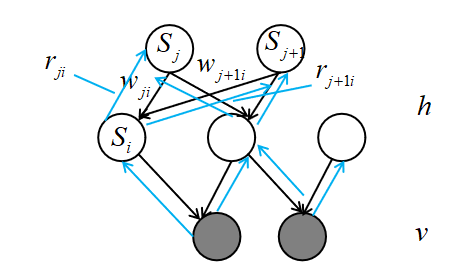
\includegraphics[width=.55\textwidth]{微信图片_20200321171927.png}
    \caption{Wake-Sleep Algorithm的模型概率图}
    \label{fig:my_label_1}
\end{figure}
正向的箭头为黑色的,代表正向的权重,表示为Generative Connection;反向的箭头为蓝色的,代表反向的权重,表示为Recognization Connect。每一个$w_{ji}$都对应一个$r_{ji}$,$w_ji$是模型中本来就存在的,而$r_{ji}$是本来并不存在的,是我们假设它存在的。

算法可以分为两个流程:
\begin{enumerate}
    \item \textbf{Wake phase: }这是一个从底向上的过程,根据有向图中D-Separation中的Tail to Tail原则,可以看到,bottom to up这样采样,所有的节点都是条件独立的,计算起来非常简单。
    \begin{enumerate}
        \item 从Bottom to up的次序来采样激活来得到每一层的样本。同样,还是假设每一个节点$S_i$是二值分布,节点之间的概率关系,仍然和Sigmoid函数相关。
        \item 有了样本之后,那就好办了。我们可以拿这些样本去训练Generative Connection,也就是求$w$。
    \end{enumerate}
    \item \textbf{Sleep phase:}这是一个从上往下的过程。
    \begin{enumerate}
        \item 从上往下来采样以得到各个节点的样本,有向图的采样非常简单。那么,\textbf{这样从上往下进行采样,得到$h,v$的样本都是虚拟出来的。因为,没有把$v$当成是可观测节点,所有不存在explain away的问题。}和Wake phase很大的不同点就在于,Wake phase是根据真实的数据$v$衍生出来的。
        \item 获得了样本之后,我们就需要去学习Recognization Connection,也就是求$r$。
    \end{enumerate}
\end{enumerate}

这并不是一个非常严谨的算法,我们叫它启发式算法,说是启发式算法,我们就已经承认了它并没有那么严密。他是通过引入了一个额外的Recognization Connection去近似一个后验分布。用一个简单分布$q(h|v)$去近似后验分布$p(h|v)$。前面,我们提到了可以把\textbf{后验分布看成是函数},那么$q(h|v)$这个函数的参数就是$r$。如果,我们将模型看成是一神经网络的话,$q(h|v)$就是一个随机的网络。如何我们将后验分布看成是一个函数的话,直接包装成一个黑箱就避免了复杂的分解过程。

~\\

老师在这里指出来,讲解醒眠算法的原因是,它虽然精度不高,但是非常有启发性,后面将讲述的很多算法,都可以很醒眠算法进行类比,从而得到启发。这里讲完,大家对醒眠算法的做法有了初步的了解,但是为什么这样做,一定还是有点懵逼的。下一小节,我们看看$w$和$r$是怎么learning到的,从而挖掘一下其背后的思想。

\subsection{$w$和$r$的Learning}
$w$和$r$的Learning过程,仍然是像之前一样使用梯度上升的方法来max Likelihood function?如果不是,那怎么操作?和KL Divergence之间又有什么联系?这就是这一小节将要解决的问题。

主要想法就是构建一个Recognization Connection去近似后验分布$p(h|v)$。聪明的同学已经观测到了,如果采用蓝色的箭头,bottom to up这样进行采样,那么根据D-Separation中的Tail to Tail,父亲节点已知的情况下,子节点都是相互独立的,那么概率图模型就是可分解的了。那么,计算就可以被简化了,我们用一个可分解的后验分布去近似一个不可分解的后验分布。

很显然,这样做,精度的误差是很大的,实际上week-sleep算法追求的不是精度而是效率,什么意思呢?用一个可分解的后验分布去近似一个不可分解的后验分布,计算量肯定会变小很多。

~\\

那么,接下来给出两个model的模型表示:

Generative Model: $P_\theta(v,h)$,$\theta = w$;

Recognization Model:$Q_\phi(h|v)$,$\phi = r$。

下一步,要求解的就是,这么Learning过程怎么Learn?目标函数是什么?

\subsubsection{Wake phase}
简单的说。第一步,首先通过bottom up生成样本;第二步,再通过这些样本来进行Learning Generative Model,求$\theta$($w$)。\textbf{Wake phase就是bottom to up生成样本,利用样本从上往下(图1)来学习$P_\theta(v,h)$的参数。}
样本来自bottom to up的过程,即为$Q_\phi(h|v)$中采样得到的,Learning可以理解为使样本使模型的值最大。也就是在$Q_\phi(h|v)$得到的样本下$P_\theta(v,h)$的值最大。所以目标函数可以被写做:
\begin{equation}
    \mathbb{E}_{Q_\phi(h|v)}[\log P_\theta(v,h)] \approx \frac{1}{N} \sum_{i=1}^N \log P_\theta(v,h)
\end{equation}
在求解$\theta$时,假设$\phi$是已知的(因为已经从这个分布中采到了样本):
\begin{equation}
    \hat{\theta} = \arg\max_\theta \mathbb{E}_{Q_\phi(h|v)}[\log P_\theta(v,h)]
\end{equation}
$\phi$初始是一个随机的分布。

\begin{table}[H]
    \centering
    \begin{tabular}{l}
    \hline
    注意到,前面有讲过近似推断的求后验的方法,这里做一个类比。
    \\
    $\log P(X) = \mathrm{ELBO} + \mathbb{KL}(q||p)$ \\
    $\mathrm{ELBO} = \mathcal{L} = \mathbb{E}_{q(h|v)} \left[ \log\frac{p(h,v)}{q(h|v)}\right] = \mathbb{E}_{q(h|v)} \left[ \log p(h,v) \right] + \mathrm{H}(q(h|v))$\\
    \hline
    \end{tabular}
    \label{tab:my_label}
\end{table}
实际上$\mathbb{E}_{Q_\phi(h|v)}[\log P_\theta(v,h)]$就是一个ELBO,因为当$Q_\phi$是固定的情况下,$H(Q_\phi(h|v))=0$,那么,$\hat{\theta} = \arg\max_\theta \mathcal{L}(\theta)$。这个优化过程可以等价于优化:
\begin{equation}
    \mathrm{KL}(Q_\phi(h|v) || P_\theta(h|v))
\end{equation}

\subsubsection{Sleep phase}
防止大家忘记,在这里给出一个详细的推导。前面过程都是一样的,不再做过多的描述,目标函数为:
\begin{equation}
    \hat{\phi} = \arg\max_\phi \mathbb{E}_{\log P_\theta(v,h)}[Q_\phi(h|v)],\quad \mathrm{fixed}\ w 
\end{equation}
在推导过程中遇到常数,添加和减少都是没有关系的。那么:
\begin{equation}
    \begin{split}
        \hat{\phi} = & \arg\max_\phi \mathbb{E}_{ P_\theta(v,h)}[Q_\phi(h|v)] \Longleftrightarrow \arg\max_\phi \mathbb{E}_{ P_\theta(v,h)}[\log Q_\phi(h|v)]\\
        = & \arg\max_\phi \int P_\theta(v,h) \log Q_\phi(h|v) dh \\
        = & \arg\max_\phi \int P_\theta(v) P_\theta(h|v) \log Q_\phi(h|v) dh \\
    \end{split}
\end{equation}
这里的$P_\theta(v)$和$\phi$和$h$都没有关系,可以看成是一个常数,所以可以直接忽略掉:
\begin{equation}
    \hat{\phi} = \arg\max_\phi \int P_\theta(h|v) \log Q_\phi(h|v) dh
\end{equation}
推导到这怎么接着进行呢?观察到因为$\theta$是已知的,所以$P_\theta(h|v)$和$\phi$没有关系。那么:
\begin{equation}
    \begin{split}
        \hat{\phi} = & \arg\max_\phi \int P_\theta(h|v) \log Q_\phi(h|v) dh \\
        = & \arg\max_\phi \int P_\theta(h|v) \log \frac{Q_\phi(h|v)}{P_\theta(h|v)} dh \\
        = & \arg\max_\phi - \mathrm{KL}(P_\theta(h|v) || Q_\phi(h|v)) \\
        = & \arg\min_\phi \mathrm{KL}(P_\theta(h|v) || Q_\phi(h|v)) \\
    \end{split}
\end{equation}

通过以上的推导,可以证明,确实可以将目标函数看成是一个ELBO,从而转换为求KL Divergence的最小化。按照同样的方法,得到公式(23)。

\subsubsection{结论分析}
通过上述的分析,看到Wake phase和Sleep phase中的目标函数,分别为:
$\mathrm{KL}(Q_\phi(h|v) || P_\theta(h|v))$和$\mathrm{KL}(P_\theta(h|v) || Q_\phi(h|v))$。两个过程求得的KL散度是相反的,有点基础的同学应该知道\textbf{KL散度不对称,不是一个距离}。

\textbf{两个过程的目标函数不一致,所以这是一个启发性算法,并不可以保证收敛。}Sleep过程,可以看成不清醒,所以目标函数都搞错了。Sleep样本是从Generative Connect过程中采样出来的,而\textbf{Model是对数据的一种假设}。个人对算法的理解请看总结。


\section{总结}
本章节的思路其实和前面的章节都很类似,实际上有的同学已经有感觉了,这个讲解的过程就是算法的孕育和成长的过程。出现了一个问题,这个问题之前的算法无法有效的解决,针对这个问题设计一个算法,这个算法可以有效的改善这个问题的求解。这个算法在求解的过程中又遇到了什么样的问题,我们如何去解决这个问题,这就是一个算法的发展过程。

首先是讲解了Sigmoid Belief Network的思想来源,将无向图变成有向图的结构则有更好的因果(causal)形式,其中未观察变量被看作观察变量发生的原因。然后介绍了模型的表示方法。紧接着在模型求解的过程中,发现由于D-Separation中的Head to Head问题,会造成节点之间的关系复杂,无法用条件独立性分解,也就是Explain away现象。这样后验分布的精确计算是intractable的。所以,Neal提出了基于MCMC的求解方法,但是MCMC只能求解小规模的图,大规模的图中会出现Mixing time过长的问题,根本就不work。

这时诞生了Wake-Sleep算法来近似推断,其主要思想就是用一个简单的分布来近似后验分布。为了解决Explain away现象,采用的是反过来求的思路,将Head to Head变成Tail to Tail就可以解决这个问题了。然后两者相互迭代,相互利用数据,来使两者的数据慢慢的逼近,\textbf{这是不是有点像GAN的思想},实际上GAN的思想就有借鉴于Wake-Sleep算法。但是,因为KL散度并不是一个距离,所以Wake-Sleep算法两个过程的目标函数是不一致的,算法并不收敛。这个算法是启发式的算法,而且很重要,后面很多算法的思想都可以和Wake-Sleep算法进行对比。




\end{document}